
%(BEGIN_QUESTION)



\paragraph{PLS programmering av innbruddsalarmanlegg}

\vskip 10pt
Du skal programmere styringen av et innbruddsalarm for et hus. Anlegget består av to sløyfer: en med magnetkontakter på dører og en med bevegelsesdetektorer i rom. Anlegget slås av med en nøkkelbryter innenfor hoveddøren. 

\vskip 10pt
Virkemåte:\\

Når anlegget aktiveres med nøkkelbryter har en 15s på å kommes seg ut før anlegget aktiveres. Når en skal inn i huset vil en bryte sløyfen med magnetkontakter, da har en 15s på seg å slå av anlegget med nøkkelbryteren. 

\vskip 10pt
Om sløyfen med PIR detektorer blir aktivert skal alarmen aktiveres direkte 

\vskip 10pt
\begin{tabular}{|c|l|c|}
\hline 
	IO-liste: & &  \tabularnewline 
\hline 
	DI0 &	 Nøkkelbryter NO(lukket i På stilling) 	 &(Inngang)\tabularnewline

\hline 
	DI1 &	 Sløyfe med magnetkontakter NC		 &(Inngang)\tabularnewline

\hline 
	DI2 &	 Sløyfe med PIR detektorer NC		 &(Inngang)\tabularnewline

\hline 
	DO2 &	 Alarm aktiv lys			 &(Utgang)\tabularnewline

\hline 
	DO2 &	 Alarm deaktivert lys			 &(Utgang)\tabularnewline

\hline 
	DO2 &	 Alarmsirene				 &(Utgang)\tabularnewline

\hline 


\end{tabular}
%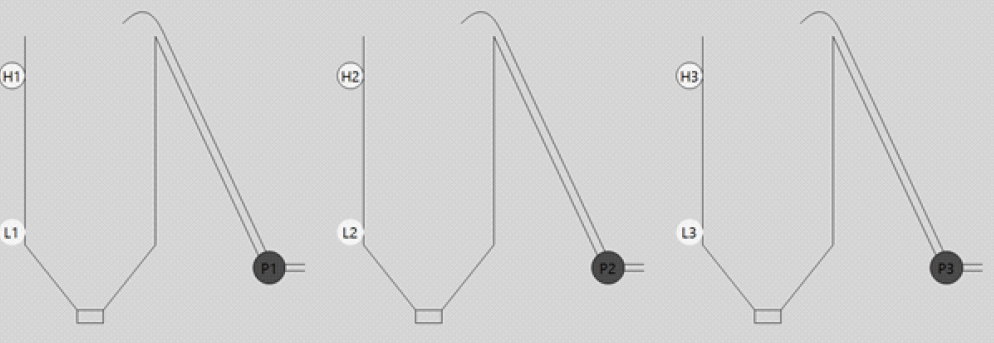
\includegraphics[width=1\textwidth]{i08012x02.png}

\vskip 10pt
\underbar{file i08014}
%(END_QUESTION)





%(BEGIN_ANSWER)
Det er ikke svar på denne oppgave
%(END_ANSWER)





%(BEGIN_NOTES)


%INDEX% PLC, programming, kombinatorisk, alarmanlegg

%(END_NOTES)




